\section{Results\label{results}}

We illustrate the behaviour of the MG preconditioner for GPUs described so far,
which exploits the INVK sparse approximate inverse solver. This approximate
inverse is obtained by the inversion of triangular
factors based on a positional drop strategy~\cite{vanDuin:99,BERTACCINI2016693}.
In particular, we show the results obtained on a linear system
arisen from a groundwater modelling application developed at the
J\"ulich Supercomputing Centre (JSC), concerning the numerical simulation
of the filtration of 3D incompressible single-phase flows through
anisotropic porous media. It is an elliptic equation with no flow
boundary conditions;  the linear systems stem from the discretization
of the equation performed by a cell-centered finite column scheme
(two-point flux approximation) on a Cartesian grid, with nonzero
entries distributed over seven diagonals. In these tests, we will
consider a homogeneous permeability tensor;  this application comes
from the framework of the Horizon 2020 EoCoE Project (Grant
676629). The equations are discretized over the unit cube; the
computational domain is partitioned by repeated sectioning along
coordinate planes. 

We performed weak scalability tests using approximately 2 millions
equations per process; thus  the total dimension ranges from 2
millions up to 256 millions equations. 

The experiments were performed on  the JURECA supercomputer at JSC.
Each GPU compute node consists
of two NVIDIA Tesla K80 GPUs with a dual-GPU design, for a total of
four available GPU devices per compute nodes.   
We used PSBLAS 3.5 (combined with its extension plugin for extended
matrix formats and GPU plugin) and MLD2P4 2.1 (combined with AINV
plugin),  compiled with  GNU compilers (C and Fortran) version 5.4.0,
MVAPICH2 version 2.3 and with CUDA 8.0.61. 

The linear systems are solved using the Conjugated Gradient (CG) method.
The stopping criterion is based on the ratio between the 2-norms of the
residual and the right-hand side vectors: the method halts if this ratio becomes smaller than $10^{-6}$).
CG is used in conjunction with a V-cycle preconditioner, for
which we consider two different configurations. In the first case the
V-cycle preconditioner applies, as pre- and post-smoother, 1 sweep of
the block-Jacobi method with INVK as a solver. In the
second configuration it applies, as pre- and post-smoother,, 2 sweep
of the Jacobi solver. In both cases, we use 10 sweeps of Block Jacobi with INVK  as
coarsest level solver.   The multilevel hierarchy is built with a
decoupled smoothed aggregation algorithm. 

For each configuration, we ran tests on CPUs only, with matrices in
CSR format, and using CPUs+GPUs, with matrices in ELLPACK format. This
allows us to quantify the gain in efficiency in using GPUs.   


\begin{figure}
\begin{center}
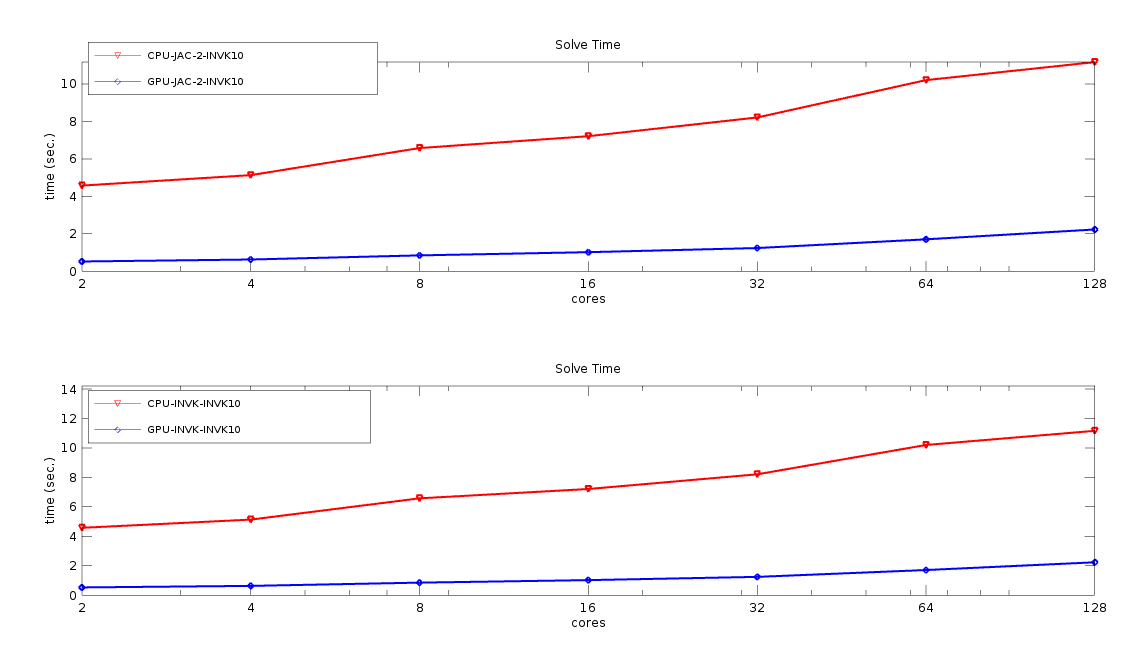
\includegraphics[width=\textwidth]{graf_solve_1.png}
\end{center}
\caption{Weak scalability, solve time\label{fig:solve_time}}
\end{figure}
The graphs in Fig.~\ref{fig:solve_time} depict the solution time for
both CPU and GPU versions; they show a relatively flat 
behaviour up until 64 nodes for both JAC-INVK and INVK-INVK variants,
and can be considered quite satisfactory in terms of weak scalability.
However, a more detailed analysis is necessary to fully elucidate the
behaviour of the application. 

\begin{figure}[h!]
\centering
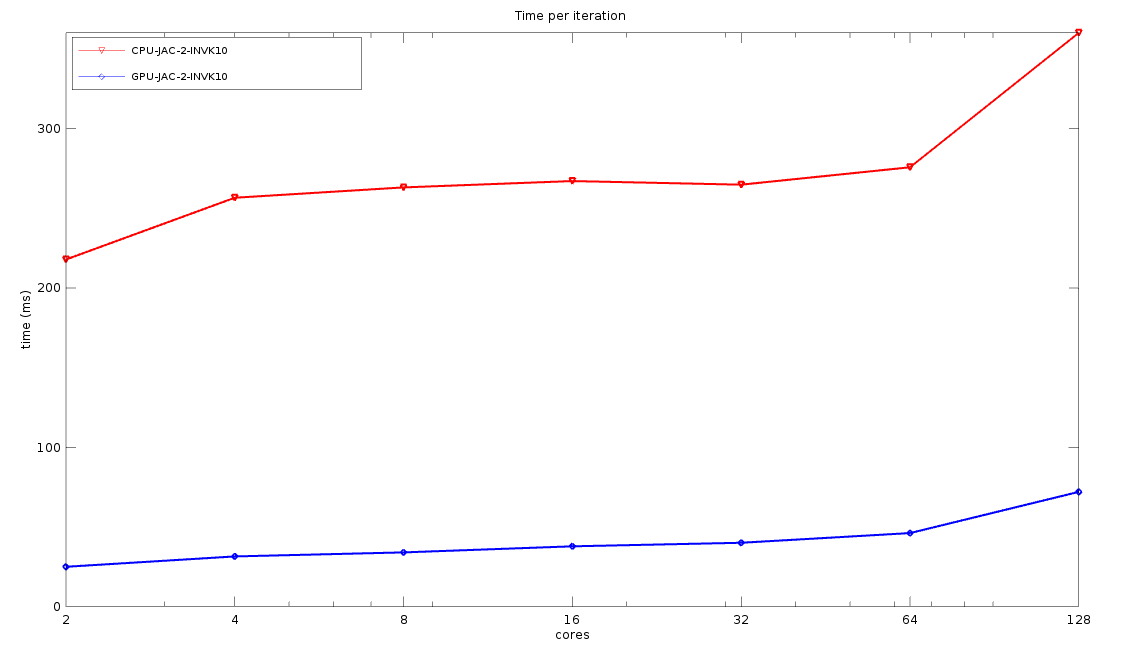
\includegraphics[width=1\textwidth]{graf_time_per_it3a.png}
\caption{Jacobi-INVK, time per iteration\label{fig:time_per_it_a}}
\end{figure}

\begin{figure}[h!]
\centering
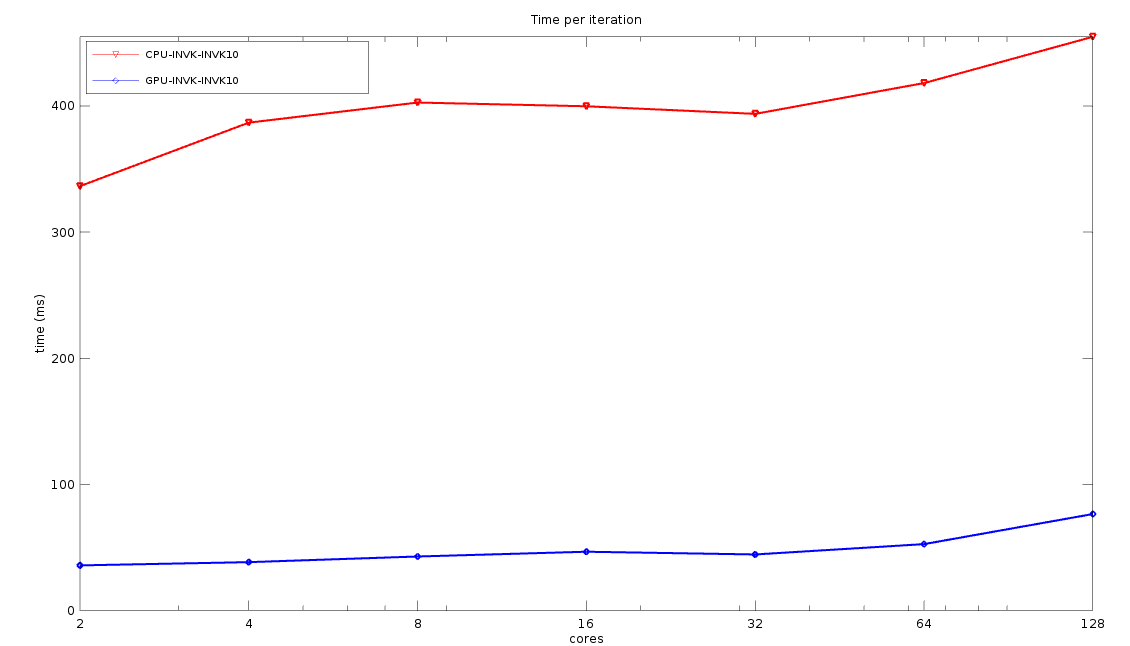
\includegraphics[width=1\textwidth]{graf_time_per_it3b.png}
\caption{INVK-INVK, time per iteration\label{fig:time_per_it_b}}
\end{figure}

In Figures~\ref{fig:time_per_it_a} and~\ref{fig:time_per_it_b}
we see that the time per iteration with the GPUs has a very flat profile between 2
and 64 nodes; this reflects a very good weak scalability within each
iteration of the method.

 However to translate this into a flat
solution time it is necessary that the number of iterations remains
constant; let us then turn our attention to the Tables~\ref{gpu-invk}
and~\ref{gpu-jac}. In the tables, we show 
respectively the number of processing elements (CPU cores or GPU
devices), the number of levels in the multilevel hierarchy, the time
for setup in seconds, then the time to solution and time per iteration
(in seconds and milliseconds), for CPUs and GPUs respectively; finally,
we show the solution speedup. The time 
to setup is essentially identical, because  almost all the
setup process is currently executed  on CPUs; in all cases, the number
of iterations to convergence is identical on CPUs and GPUs. 

There are two lines for the tests at 128 devices in each table. 
The first line is obtained by letting the aggregation algorithm run with
default arguments; in this case the preconditioner uses a hierarchy
with 5 levels and achieves a number of iterations equal to or less than
that for 32 and 64 devices, but because there are 5 levels, the time
per iteration deteriorates.  In the second line, we force the
preconditioner to use 4 levels, in which case the time per iteration
remains essentially constant on the GPU and very close on the CPU, but
the number of iterations increases. In both
configurations the best solution time on the GPU is obtained with 4
levels, whereas the CPU version is faster with 5 levels. 

In summary, the aggregation algorithm is capable of obtaining very
good algorithmic scalability, but in some cases at the expense of time
per iteration, so that it does not necessarily correspond to the best 
solution time. 
Additional work will be required to design aggregation
strategies capable of obtaining a better trade-off with as little user
intervention as possible; some possible directions are outlined
in~\cite{bcm-toms}.  




\iffalse
\begin{table}[h!]
\centering
\caption{Numerical results for CG + ML preconditioner, runs on CPUs, with 1 sweep of BJAC(INVK) as smoother on inner levels.}
\label{cpu-invk}

\begin{tabular}{rrrrrrr}
% \multicolumn{1}{l}{np} & \multicolumn{1}{l}{levels} &   \multicolumn{1}{l}{Iters} & \multicolumn{1}{l}{\begin{tabular}[c]{@{}l@{}}Prec    \\  
%  time (s)\end{tabular}} &
%                           \multicolumn{1}{l}{\begin{tabular}[c]{@{}l@{}}Solve  \\  
% Time (s)\end{tabular}} &
%                          \multicolumn{1}{l}{\begin{tabular}[c]{@{}l@{}}Time per \\ 
% Iteration (ms)\end{tabular}} & \multicolumn{1}{l}{\begin{tabular}[c]{@{}l@{}}Total  \\   Time (s)\end{tabular}} \\ \hline
NP  & Levels & Iters & Tsetup & Tsolve & T/iter & Ttotal \\
    &        &       & (s)    & (s)    & (ms)   & (s)    \\
\hline
1   & 4       & 14  & 17.74 & 4.42  & 320      & 22.15   \\
2   & 4       & 15  & 19.43 & 5.05  & 340      & 24.47   \\
4   & 4       & 18  & 21.85 & 6.96  & 390      & 28.81   \\
8   & 4       & 20  & 28.32 & 8.05  & 400      & 36.37   \\
16  & 4       & 24  & 26.38 & 9.59  & 400      & 35.98   \\
32  & 4       & 29  & 23.52 & 11.42 & 390      & 34.93   \\
64  & 4       & 34  & 29.61 & 14.21 & 420      & 43.82   \\
128 & 5       & 29  & 28.39 & 13.19 & 450      & 41.58    \\
\hline
\end{tabular}
\end{table}

\begin{table}[h!]
\centering
\caption{Numerical results for CG + ML preconditioner, runs on GPUs, with 1 sweep of BJAC(INVK) as smoother on inner levels.}
\label{gpu-invk}

\begin{tabular}{rrrrrrrr}
% \multicolumn{1}{l}{np} & \multicolumn{1}{l}{levels} & \multicolumn{1}{l}{It} & \multicolumn{1}{l}{\begin{tabular}[c]{@{}l@{}}Prec    \\   time (s)\end{tabular}} & \multicolumn{1}{l}{\begin{tabular}[c]{@{}l@{}}Solve  \\  Time (s)\end{tabular}} & \multicolumn{1}{l}{\begin{tabular}[c]{@{}l@{}}Time per \\ Iteration (ms)\end{tabular}} & \multicolumn{1}{l}{\begin{tabular}[c]{@{}l@{}}Total  \\   Time (s)\end{tabular}} & \multicolumn{1}{l}{\begin{tabular}[c]{@{}l@{}}Speed up\\ cpu/gpu\end{tabular}} \\ \hline
NP  & Levels & Iters & Tsetup & Tsolve & T/iter & Ttotal & Speedup\\
    &        &       & (s)    & (s)    & (ms)   & (s)   &  \\
\hline
1   & 4       & 14  & 18.80 & 0.45 & 30   & 19.24& 9.92  \\
2   & 4       & 15  & 20.55 & 0.54 & 40   & 21.09& 9.40  \\
4   & 4       & 18  & 22.84 & 0.69 & 40   & 23.54& 10.08 \\
8   & 4       & 20  & 29.18 & 0.86 & 40   & 30.03& 9.40  \\
16  & 4       & 24  & 27.38 & 1.12 & 50   & 28.50& 8.57  \\
32  & 4       & 29  & 23.74 & 1.29 & 40   & 25.02& 8.85  \\
64  & 4       & 34  & 30.53 & 1.79 & 50   & 32.32& 7.94  \\
128 & 5       & 29  & 29.48 & 2.22 & 80   & 31.70& 5.94  \\
\hline
\end{tabular}
\end{table}

\begin{table}[h!]
\centering
\caption{Numerical results for CG + ML preconditioner, runs on CPUs, with 2 sweeps of JACOBI as smoother on inner levels.}
\label{cpu-jac}

\begin{tabular}{rrrrrrr}
% \multicolumn{1}{l}{np} & \multicolumn{1}{l}{levels} & \multicolumn{1}{l}{It} & \multicolumn{1}{l}{\begin{tabular}[c]{@{}l@{}}Prec    \\   time (s)\end{tabular}} & \multicolumn{1}{l}{\begin{tabular}[c]{@{}l@{}}Solve  \\  Time (s)\end{tabular}} & \multicolumn{1}{l}{\begin{tabular}[c]{@{}l@{}}Time per \\ Iteration (s)\end{tabular}} & \multicolumn{1}{l}{\begin{tabular}[c]{@{}l@{}}Total  \\   Time (s)\end{tabular}} \\ \hline
NP  & Levels & Iters & Tsetup & Tsolve & T/iter & Ttotal \\
    &        &       & (s)    & (s)    & (ms)   & (s)    \\
\hline
1   & 4       & 19  & 2.83  & 3.76  & 200   & 6.59    \\
2   & 4       & 21  & 3.65  & 4.57  & 220   & 8.23    \\
4   & 4       & 20  & 4.21  & 5.13  & 260   & 9.35    \\
8   & 4       & 25  & 4.75  & 6.58  & 260   & 11.33   \\
16  & 4       & 27  & 4.97  & 7.21  & 270   & 12.18   \\
32  & 4       & 31  & 4.88  & 8.21  & 260   & 13.09   \\
64  & 4       & 37  & 5.79  & 10.20 & 280   & 16.00   \\
128 & 5       & 31  & 6.72  & 11.16 & 360   & 17.88  \\
\hline
\end{tabular}
\end{table}

\begin{table}[h!]
\centering
\caption{Numerical results for CG + ML preconditioner, runs on GPUs, with 2 sweeps of JACOBI as smoother on inner levels.}
\label{gpu-jac}
\begin{tabular}{rrrrrrrr}
% \multicolumn{1}{l}{np} & \multicolumn{1}{l}{levels} & \multicolumn{1}{l}{It} & \multicolumn{1}{l}{\begin{tabular}[c]{@{}l@{}}Prec    \\   time (s)\end{tabular}} & \multicolumn{1}{l}{\begin{tabular}[c]{@{}l@{}}Solve  \\  Time (s)\end{tabular}} & \multicolumn{1}{l}{\begin{tabular}[c]{@{}l@{}}Time per \\ Iteration (s)\end{tabular}} & \multicolumn{1}{l}{\begin{tabular}[c]{@{}l@{}}Total  \\   Time (s)\end{tabular}} & \multicolumn{1}{l}{\begin{tabular}[c]{@{}l@{}}Speed up\\ cpu/gpu\end{tabular}} \\ \hline
NP  & Levels & Iters & Tsetup & Tsolve & T/iter & Ttotal & Speedup\\
    &        &       & (s)    & (s)    & (ms)   & (s)   &  \\
\hline
1   & 4       & 19  & 3.13  & 0.40 & 20   & 3.53 & 9.39  \\
2   & 4       & 21  & 4.06  & 0.52 & 20   & 4.59 & 8.73  \\
4   & 4       & 20  & 4.65  & 0.63 & 30   & 5.28 & 8.16  \\
8   & 4       & 25  & 5.20  & 0.85 & 30   & 6.05 & 7.74  \\
16  & 4       & 27  & 5.39  & 1.02 & 40   & 6.42 & 7.06  \\
32  & 4       & 31  & 5.35  & 1.24 & 40   & 6.59 & 6.61  \\
64  & 4       & 37  & 6.25  & 1.71 & 50   & 7.96 & 5.98  \\ 
128 & 5       & 31  & 7.19  & 2.23 & 70   & 9.43 & 5.00  \\
\hline
\end{tabular}
\end{table}

\else

\begin{table}[h!]
\centering
\begin{tabular}{rrrrrrrrr}
% \multicolumn{1}{l}{np} & \multicolumn{1}{l}{levels} &
% \multicolumn{1}{l}{It} &
% \multicolumn{1}{l}{\begin{tabular}[c]{@{}l@{}}Prec    \\   time
% (s)\end{tabular}} &
% \multicolumn{1}{l}{\begin{tabular}[c]{@{}l@{}}Solve  \\  Time
% (s)\end{tabular}} &
% \multicolumn{1}{l}{\begin{tabular}[c]{@{}l@{}}Time per \\ Iteration
% (ms)\end{tabular}} &
% \multicolumn{1}{l}{\begin{tabular}[c]{@{}l@{}}Total  \\   Time
% (s)\end{tabular}} &
% \multicolumn{1}{l}{\begin{tabular}[c]{@{}l@{}}Speed up\\
% cpu/gpu\end{tabular}} \\ \hline
    &        &       &        & \multicolumn{2}{c}{CPU} & \multicolumn{2}{c}{GPU} & \\
NP  & Levels & Iters & Tsetup & Tsolve & T/iter  & Tsolve & T/iter  & Speedup\\
    &        &       & (s)    & (s)    & (ms)    & (s)    & (ms)    & GPU/CPU \\
\hline
1   & 4       & 14  & 18.80 & 4.42  & 320    & 0.45 & 30   &  9.92  \\
2   & 4       & 15  & 20.55 & 5.05  & 340    & 0.54 & 40   &  9.40  \\
4   & 4       & 18  & 22.84 & 6.96  & 390    & 0.69 & 40   &  10.08 \\
8   & 4       & 20  & 29.18 & 8.05  & 400    & 0.86 & 40   &  9.40  \\
16  & 4       & 24  & 27.38 & 9.59  & 400    & 1.12 & 50   &  8.57  \\
32  & 4       & 29  & 23.74 & 11.42 & 390    & 1.29 & 40   &  8.85  \\
64  & 4       & 34  & 30.53 & 14.21 & 420    & 1.79 & 50   &  7.94  \\
128 & 5       & 29  & 29.48 & 13.19 & 450    & 2.22 & 80   &  5.94  \\
\hline
128 & 4       & 43  & 29.48 & 19.32 & 450    & 2.18 & 51   &  8.85  \\
\hline
\end{tabular}
\caption{Weak Scalability,  CG + ML preconditioner,  with 1 sweep of BJAC(INVK) smoother on inner levels.\label{gpu-invk}}
\end{table}


\begin{table}[h!]
\centering
\begin{tabular}{rrrrrrrrrrr}
% \multicolumn{1}{l}{np} & \multicolumn{1}{l}{levels} & \multicolumn{1}{l}{It} & \multicolumn{1}{l}{\begin{tabular}[c]{@{}l@{}}Prec    \\   time (s)\end{tabular}} & \multicolumn{1}{l}{\begin{tabular}[c]{@{}l@{}}Solve  \\  Time (s)\end{tabular}} & \multicolumn{1}{l}{\begin{tabular}[c]{@{}l@{}}Time per \\ Iteration (s)\end{tabular}} & \multicolumn{1}{l}{\begin{tabular}[c]{@{}l@{}}Total  \\   Time (s)\end{tabular}} & \multicolumn{1}{l}{\begin{tabular}[c]{@{}l@{}}Speed up\\ cpu/gpu\end{tabular}} \\ \hline
    &        &       &        & \multicolumn{2}{c}{CPU} &\multicolumn{2}{c}{GPU} & \\
NP  & Levels & Iters & Tsetup & Tsolve & T/iter & Tsolve & T/iter  & Speedup\\
    &        &       & (s)    & (s)    & (ms)   & (s)    & (ms)    & GPU/CPU \\
\hline
1   & 4       & 19  & 3.13  & 3.76  & 200 & 0.40 & 20   & 9.39  \\
2   & 4       & 21  & 4.06  & 4.57  & 220 & 0.52 & 20   & 8.73  \\
4   & 4       & 20  & 4.65  & 5.13  & 260 & 0.63 & 30   & 8.16  \\
8   & 4       & 25  & 5.20  & 6.58  & 260 & 0.85 & 30   & 7.74  \\
16  & 4       & 27  & 5.39  & 7.21  & 270 & 1.02 & 40   & 7.06  \\
32  & 4       & 31  & 5.35  & 8.21  & 260 & 1.24 & 40   & 6.61  \\
64  & 4       & 37  & 6.25  & 10.20 & 280 & 1.71 & 50   & 5.98  \\ 
128 & 5       & 31  & 7.19  & 11.16 & 360 & 2.23 & 70   & 5.00  \\
\hline
128 & 4       & 46  & 7.00  & 14.05 & 305 & 2.04 & 44   & 6.88  \\
\hline
\end{tabular}
\caption{Weak Scalability,  CG + ML preconditioner,  with 2 sweeps of JACOBI smoother on inner levels.\label{gpu-jac}}
\end{table}
\fi

% When GPUs are used, the last column shows the speed-up of the solver
% phase on the gpu with respect to the cpu solve time.
The GPU/CPU speed-up achieves a maximum value of 10 in the case of 8
processes and it achieves a value between  5 and 9  with 128
processes. The  increasing number of levels leads to a decrease in
the size of the coarsest level matrix which affects performance for
two reasons, first because the matrices at the coarse level are too
small to make good use of the GPU device computational power, and also
because the communication to computation ratio gets worse.


% \begin{figure}[h!]
% \caption{Time per iteration}
% \centering
% 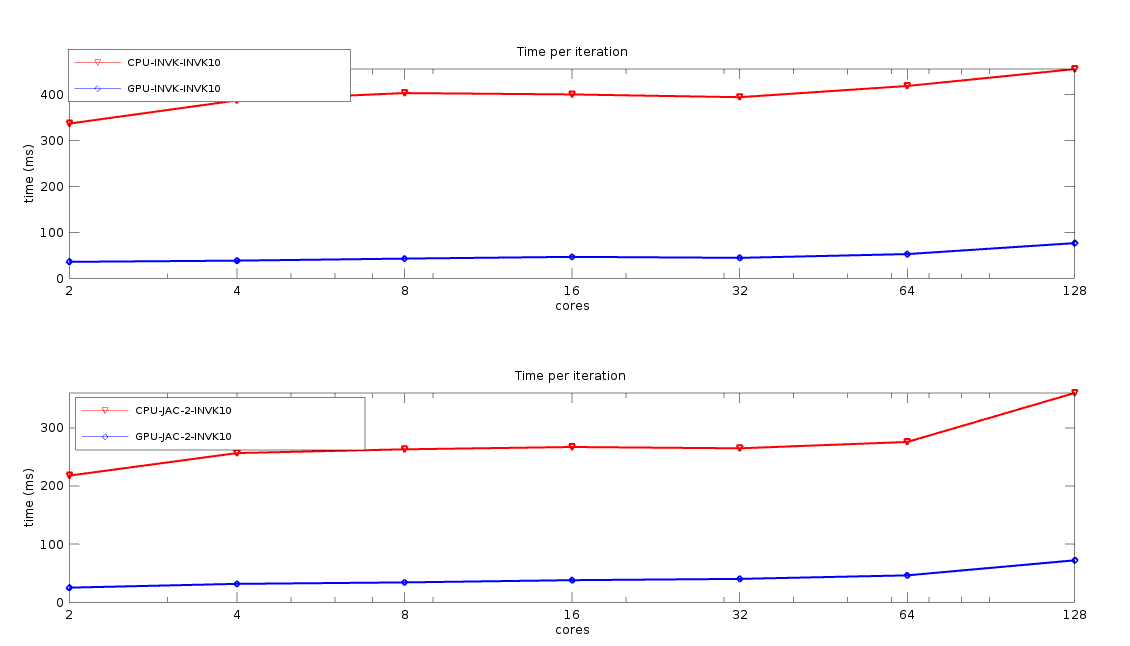
\includegraphics[width=1\textwidth]{time_per_it.png}
% \label{fig:time_per_it}
% \end{figure}


% \begin{figure}
% \begin{center}
% 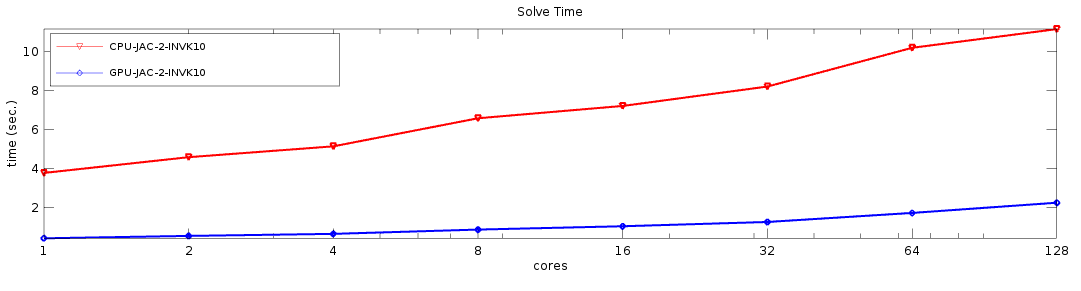
\includegraphics[width=.9\textwidth]{graf_jac2.png}
% \end{center}
% \caption{JAC2-INVK}
% \end{figure}
